    The major axis of a conic is the chord which passes through the vertices of the conic.
    The direction vector of the major axis in this case is
    \begin{align}
        \vec{P}_2-\vec{P}_1 \equiv \vec{e}_1 = \vec{n}
\label{eq:chapters/11/11/4/13/6/n} 
    \end{align}
    which is the normal vector for the directrix.
    Since $e > 1$, the conic is a hyperbola.
Substituting  
\eqref{eq:chapters/11/11/4/13/6/n} 
in
  \eqref{eq:conic_quad_form_v},
\eqref{eq:conic_quad_form_u}
and
\eqref{eq:conic_quad_form_f},
\begin{align}
	\vec{V} = \myvec{1-e^2&0\\0&1} = \myvec{-\frac{7}{9}&0\\0&1} \label{eq:chapters/11/11/4/14/6} 
\end{align}
    The centre of the hyperbola is 
\begin{align}
	\vec{c} = \frac{\vec{P}_1+\vec{P}_2}{2} = \vec{0} = \vec{u}
\end{align}
from \eqref{eq:conic_parmas_c_def}.      Substituting $\vec{P}_1$ and $\vec{P}_2$ in 
    \eqref{eq:conic_quad_form},
    \begin{align}
        \vec{P}_1^\top\vec{VP}_1 + 2\vec{u}^\top\vec{P}_1 + f &= 0 \label{eq:chapters/11/11/4/14/ep1} \\
        \vec{P}_2^\top\vec{VP}_2 + 2\vec{u}^\top\vec{P}_2 + f &= 0 \label{eq:chapters/11/11/4/14/ep2}
	\\
	    \implies f = \vec{P}_1^\top\vec{VP}_1  = 49\brak{e^2-1}&=\frac{343}{9}
    \end{align}
    upon adding 
    \eqref{eq:chapters/11/11/4/14/ep2} and \eqref{eq:chapters/11/11/4/14/ep1}
    and simplifying.
    Therefore, the equation of the conic is
    \begin{align}
        \vec{x}^\top\myvec{-\frac{7}{9}&0\\0&1}\vec{x} + \frac{343}{9} = 0
    \end{align}
See \figref{fig:chapters/11/11/4/14/hyperbola}.
    \begin{figure}[H]
        \centering
        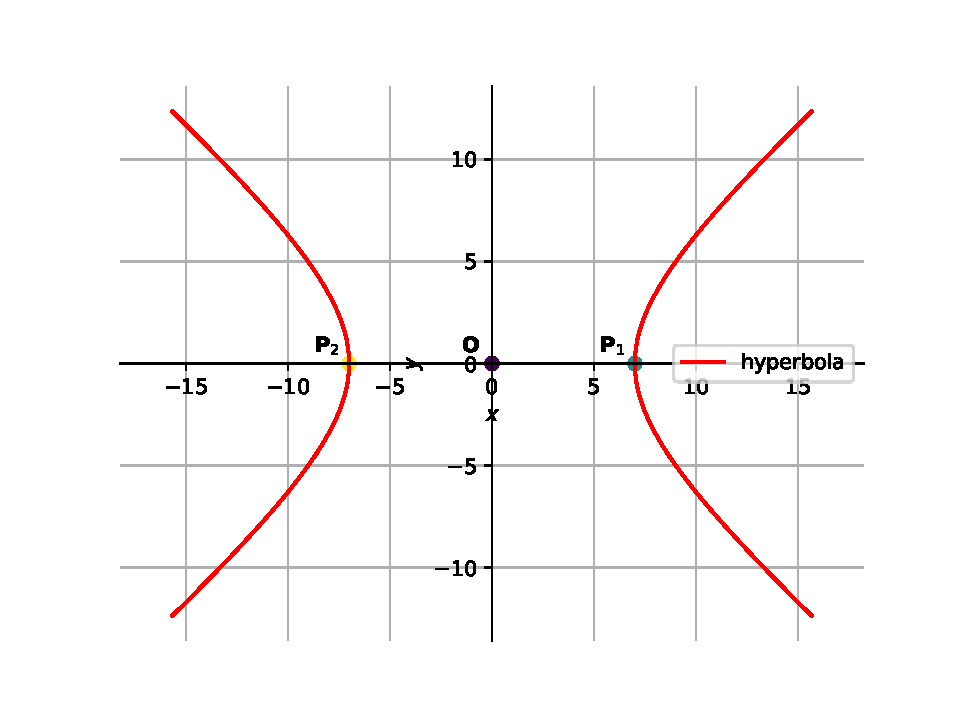
\includegraphics[width=0.75\columnwidth]{chapters/11/11/4/14/figs/fig.pdf}
        \caption{}
        \label{fig:chapters/11/11/4/14/hyperbola}
    \end{figure}
